% =====================================================================
% main.tex -- rewritten draft (2026-09-28). Replaces the 2026-09-20 draft
% (E:\flybrain_e5a_v3_20260920\main.tex, kept unchanged as a record).
% Why the rewrite: see mechanism/PAPER_OVERTURN_20260928.md.
% Every number below comes from mechanism/RESULTS_20260928.md and the JSON
% files it names (E:/mechanism_20260928/).  Figures: make_figures.py.
% Not compiled locally (no LaTeX on this machine).
% =====================================================================
\documentclass[conference]{IEEEtran}
\usepackage{amsmath,amssymb,graphicx,booktabs,url,xcolor}
\usepackage[utf8]{inputenc}
\newcommand{\pending}[1]{\textcolor{red}{[#1]}}
\newcommand{\todo}[1]{\textcolor{blue}{[TODO: #1]}}

\begin{document}

\title{Three Addresses of a Connectome-Constrained Mushroom-Body Memory:
Dopamine Chooses the Compartment, Sparse Kenyon-Cell Codes Set the Cue,
Side- and Subtype-Specific Routing Shapes the Output}

\author{\IEEEauthorblockN{First Author}\IEEEauthorblockA{Institution}}

\maketitle

% =====================================================================
\begin{abstract}
We asked which constraints of the mushroom-body (MB) wiring determine where a
dopamine-gated memory is stored, how it is read out, how long it lasts, and
how it reaches the rest of the brain, using a leaky integrate-and-fire model of
a whole adult male \textit{Drosophila} CNS connectome (166{,}700 neurons) with
local plasticity on its 61{,}210 Kenyon-cell (KC) to MB-output-neuron (MBON)
synapses. A validated snapshot-and-transplant interface shows that, from about
one second after a write, the memory is carried entirely by the KC$\rightarrow$MBON
weights: swapping the fast network state changes nothing, and the fast state
relaxes with the single-neuron membrane time constant, with no reverberation.
Retention is set entirely by the prescribed synaptic decay; removing the decay
leaves the readout unchanged for over two minutes. The readout depends
critically on input sparseness. At the input density used in earlier work
(512 of 675 projection neurons per symbol), 87\% of KCs respond to every probe
and the KC sets of different symbols overlap with Jaccard index 0.93, so the MB
behaves as one decaying scalar store per MBON. At sparse input (160--192
projection neurons; 9--16\% of KCs active; Jaccard 0.08--0.14), readout becomes
cue-specific (the written item reads out 3.6--4.7 times more strongly than
other probes, median over six pairs) and depends on KC identity: scrambling
which KCs carry the written change, while preserving every MBON's weight
changes exactly, removes 34--89\% of the cued readout. Cue specificity needs
only sparseness: random PN$\rightarrow$KC wiring reproduces it. The identity
of the output needs the real wiring, but only at two coarse levels: body side
and KC subtype. Randomising the PN$\rightarrow$KC or KC$\rightarrow$MBON wiring
makes the MBON outputs of different items nearly identical (mean pairwise
cosine 0.76 against 0.96--0.99), whereas swapping KC output profiles freely
among KCs of the same subtype and body side leaves it intact (0.75). With
side-blind symbol codes, the sparse KC threshold amplifies small differences
into lateralised storage (the left share of written KCs ranges from 0.04 to
0.95 across items); with bilaterally symmetric glomerular codes, items instead
differ in the KC subtypes they recruit ($\alpha\beta$ share $0.42\pm0.15$),
which subtype-specific KC$\rightarrow$MBON routing turns into distinct outputs
(0.88 against 0.96--0.99). With one teacher the dopamine gate is identical
across items; with different teachers (PAM subsets, PPL) the teacher decides
the compartment and explains 87\% of the output variance against 5\% for the
item. Finally, downstream neurons receive the memory only when it flips
at least one MBON spike (35 of 35 cells with changed MBON rasters against 0 of
93 with identical rasters), which makes the effective readout discrete.
\end{abstract}

% =====================================================================
\section{Introduction}
The MB stores associative memories as dopamine-gated, compartment-specific
changes of KC$\rightarrow$MBON synapses \cite{hige2015,aso2014a,modi2020}.
Its anatomy suggests a division of labour: an expansion from about 50
glomerular channels onto thousands of sparsely active KCs
\cite{honegger2011,lin2014}, apparently random at the level of
PN$\rightarrow$KC convergence \cite{caron2013}, followed by a compartmental
KC$\rightarrow$MBON layer with dopaminergic teaching signals
\cite{aso2014a,takemura2017,li2020}. Theory argues that such expansion and
connectivity degree are chosen for what the downstream plasticity must do
\cite{litwinkumar2017}.

Whole-connectome simulations make it possible to ask these questions with the
real wiring in place \cite{shiu2024,lappalainen2024}. We use such a model not to
claim a memory capacity but to localise the memory causally: which state
variable carries it, which wiring determines which cue can retrieve it and what
it evokes at the output, what sets its lifetime, and how it leaves the MB.
Each question is answered by an intervention with a matched control and, where
possible, a restoration.

An earlier analysis of this model \cite{olddraft} reported that plasticity
bought no readout advantage and that the write-effect direction was fixed by
the probe rather than the content. Section~\ref{sec:corrections} explains why
those conclusions do not stand: part of their data came from a simulator
version that wrote to the wrong synapses, two of their confirmed predictions
hold by construction, and all of their experiments ran at a dense input
operating point in which the MB's sparse code is absent.

% =====================================================================
\section{Model and Methods}
\label{sec:methods}

\subsection{Connectome and dynamics}
The substrate is an adult male \textit{Drosophila} CNS reconstruction
\todo{cite the connectome release used by the flybrain package} with 166{,}700
neurons and 25{,}582{,}938 synaptic entries, of which 25{,}088{,}107 remain
after removing inputs onto sensory neurons. Populations: 4{,}064 KCs, 97 MBONs,
356 dopaminergic neurons (PAM/PPL/PPM), 675 projection neurons (PNs) in 180
annotated types, and two APL neurons. Neurons are leaky integrate-and-fire
units ($\Delta t=20$~ms, $\tau=100$~ms, threshold 1, reset 0) driven by
$v\leftarrow e^{-\Delta t/\tau}v + g\,Wz + b$, with gain $g=1.5$, tonic input
$b=0.05$ and no intrinsic noise; only spikes $z$ propagate. APL inhibits KCs
(summed APL$\rightarrow$KC weight $\approx-190$ over $\sim$2{,}300 edges per APL)
and fires 1--2 times per input token at the legacy operating point.

\subsection{Plasticity}
Only the 61{,}210 existing KC$\rightarrow$MBON entries are plastic:
$w_{km}=w^0_{km}(1+m_{km})$, with
$m_{km}\leftarrow e^{-T/\tau_w}m_{km}+\eta\,\gamma_m a_k$ per token of length
$T=120$~ms, clipped to $|m|\le0.9$. $a_k$ is the KC's spike count in the token
divided by six, and $\gamma_m$ is a per-MBON gate computed from the simulated
dopaminergic spikes through the connectome's own DAN$\rightarrow$MBON edges with
hand-set valence signs (PAM $+1$, PPL $-1$, PPM $+0.5$). $\eta=0.02$ and
$\tau_w=16$~s unless stated. The rule, the signs and the decay are modelling
choices; results that depend on them are reported as interactions between
these choices and the wiring, not as properties of the wiring alone.

\subsection{Protocol}
Symbols are encoded as fixed random subsets of PNs (the \emph{PN code}); each
token injects the code for six steps (drive $d$ on the first step, $0.5d$
after). A write presents one symbol for 32 tokens with a dopaminergic pulse
(PAM, $+2.0$) on each token; a gap of $G$ silent tokens follows with plasticity
off and passive decay on; a probe token (drive $2.5d$) is read over six further
silent steps. Readouts are (i) pre-reset membrane voltages of the 97 MBONs and
of 256 central neurons with the largest MBON input, averaged per step over the
settle window, (ii) the write-attributable MBON input current
$I_m=\sum_k\Delta w_{km}\,c_k/6$, with $c_k$ the probe's KC spike counts, which
isolates the synaptic effect from the spiking nonlinearity, and (iii) MBON
spike rasters. The \emph{operating point} is the PN code size $n_{PN}$ (of 675)
and the drive scale; 512 at scale 1.0 is the legacy setting of earlier work.
Drive saturates above scale 1.5 because PN spiking is binary.

\subsection{Snapshot, restore and transplant}
The complete dynamical state is the voltage vector, the last spike set (the
only transmission delay), the harness spike traces, the KC eligibility trace
(inert when, as here, it does not enter the update) and the synaptic state
$(m,w)$; all other weights are hashed and verified constant. Restoring a
snapshot reproduced natural continuation to the level of the GPU's own
replay-to-replay variability (maximum absolute voltage difference
$2.4\times10^{-7}$ at MBONs against $2.4\times10^{-7}$ between natural replays),
while three injected errors were detected: $+10^{-3}$ on all MBON voltages
($\sim$1000$\times$ the floor), restoring $m$ without the matching $w$
($\sim3\times10^6\times$), and $+10^{-3}$ on a single synapse ($4$--$5\times$).

\subsection{Interventions and statistics}
Weight scrambles permute the actual weight changes $\Delta w$ (not $m$) across
edges, preserving their multiset exactly, either within each MBON (keeping each
MBON's change distribution, destroying KC identity) or within each KC (keeping
which KCs changed, destroying which MBON they address). Wiring nulls rewire
PN$\rightarrow$KC or KC$\rightarrow$MBON edges while preserving in-degrees,
out-degrees and weight multisets, without duplicate edges. The simulation is
deterministic at zero noise; the units of replication are write pairs, items
and null draws, all within one connectome, so we report ranges and medians and
do not attach $p$ values to population claims. Decision rules were written
into each script before its data were inspected.

% =====================================================================
\section{Results}

\subsection{After one second the memory is carried by the KC$\rightarrow$MBON weights}
We saved full states at the pre-probe instant of episodes that wrote item $X$
or $Y$ and transplanted the synaptic state $m$ and the fast state $s$
independently (Table~\ref{tab:m1}). With no gap, the probe response is dominated
by residual activity. From eight tokens (0.96~s) on, swapping $m$ reproduces
the entire content difference and swapping $s$ reproduces none of it, and the
same holds on a common no-write fast state. The fast-state difference between
episodes decays with $\tau\approx0.1$~s, the membrane time constant, reaching
float32 resolution by 3.84~s; no spikes remain two tokens after the write. At
this operating point the recurrent wiring does not prolong activity-based
memory. The same decomposition at sparse input (192 PNs) gives the same
result: from eight tokens on, swapping $m$ reproduces 99.9--100\% of the
content difference and swapping $s$ at most 0.6\% (Fig.~\ref{fig:m1}).

\begin{figure*}[t]\centering
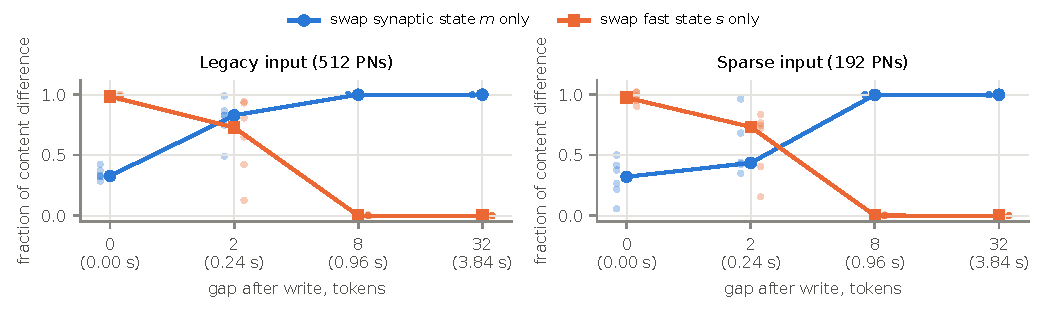
\includegraphics[width=0.95\textwidth]{figures/fig1_transplant.pdf}
\caption{Transplant decomposition. Response change at the MBON level when only
the synaptic state $m$ (circles) or only the fast state $s$ (squares) of the
episode is swapped, as a fraction of the natural content difference between
two writes. Lines: medians; faint points: individual pair $\times$ probe cells
(pairs $a/c$, $b/d$; probes: both written items and a neutral cue).}
\label{fig:m1}\end{figure*}

\begin{table}[t]
\caption{Transplant decomposition at the legacy operating point (MBON level,
pairs $a/c$ and $b/d$, probes = both items and a neutral cue). $D_m$ and $D_s$:
response change when only $m$ or only $s$ is swapped, relative to the natural
content difference.}
\label{tab:m1}\centering
\begin{tabular}{@{}lrrr@{}}\toprule
Gap & Fast-state $\lVert\Delta v\rVert$ & $D_m/D_{\mathrm{nat}}$ & $D_s/D_{\mathrm{nat}}$\\\midrule
0 & 28--31 & 0.29--0.42 & 0.97--1.00\\
2 tokens & 2.6--3.1 & 0.49--0.99 & 0.13--0.94\\
8 tokens & $\approx2\times10^{-3}$ & 1.000 & $\le0.007$\\
32 tokens & $\approx7\times10^{-6}$ & 1.000 & 0.000\\\bottomrule
\end{tabular}
\end{table}

\subsection{Retention is the prescribed decay; the readout is thresholded}
The synaptic difference between two writes follows $e^{-t/\tau_w}$ exactly for
$\tau_w\in\{4,16,64\}$~s. With the decay removed, the write effect and the
content difference at the readout stay constant for 123~s: the network's
activity contributes neither forgetting nor consolidation, because it is
silent between write and probe. The readout, however, is not a smooth image of
the trace. For $\tau_w=16$~s the content difference of one probe stays above
98\% of its initial value for 15~s and drops to 4\% by 31~s, while 16\% of the
synaptic difference remains; other probes show steps and even transient
increases. Effective readout time constants were 12--15~s for $\tau_w=16$~s,
shorter than the trace. The steps coincide with MBON spikes appearing or
disappearing (Section~\ref{sec:gating}). A retention of 38.3\% after 15.36~s,
reported earlier as a model memory lifetime, equals $e^{-15.36/16}$, the
prescribed constant.

The sparse regime makes the mechanism explicit (Fig.~\ref{fig:curve}). The
cued input current follows $e^{-t/16\,\mathrm{s}}$ exactly. The write adds one
MBON spike to the probe response (6 against 5); while that spike persists, the
MBON voltage difference and the downstream difference stay within 7\% of their
initial values, and when it disappears, between 15.4 and 30.7~s, the
downstream difference drops to the numerical floor although 16\% of the
synaptic difference remains. With the decay removed, the extra spike and the
downstream difference persist unchanged for 123~s. Probes that never flip an
MBON spike leave the downstream response at the floor throughout.

\begin{figure}[t]\centering
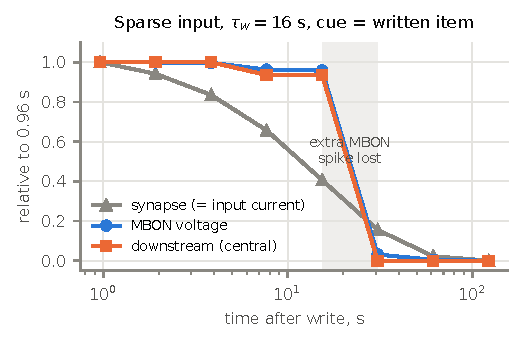
\includegraphics[width=\columnwidth]{figures/fig2_curve_gating.pdf}
\caption{Retention at sparse input (192 PNs, $\tau_w=16$~s, pair $a/c$, cue
$a$), each quantity relative to its value at 0.96~s. The synaptic difference
equals the cued input current and decays exponentially; the MBON voltage and
downstream differences track the presence of one extra MBON spike (shaded:
interval in which it is lost).}
\label{fig:curve}\end{figure}

\subsection{The legacy operating point has no sparse KC code}
At $n_{PN}=512$, 51--68\% of KCs spike in each write token and 87\% during the
probe; KC sets of different symbols overlap with Jaccard 0.55--0.67 during
writing and 0.93 during the probe. APL fires but does not sparsen this input.
Every probe therefore reads almost the same KCs, and the written trace is
accessed as a per-MBON sum. Scrambling KC identity within each MBON leaves the
readout current almost unchanged (83--88\% of its magnitude, cosine
0.99--1.00), and a neutral cue reads the stored content as strongly as the
written item (cue specificity 0.96--1.13).

Sweeping the PN code size (Table~\ref{tab:sweep}) reveals a sparse regime
between 160 and 192 PNs in which probes activate 9--16\% of KCs, symbols share
few KCs, and the write still changes MBON voltages by orders of magnitude above
the numerical floor (Fig.~\ref{fig:sweep}). Below about 128 PNs the KC layer
falls silent.

\begin{figure}[t]\centering
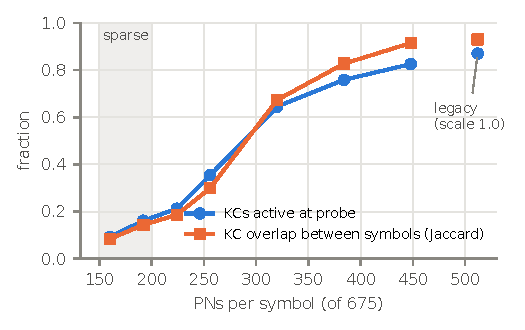
\includegraphics[width=\columnwidth]{figures/fig3_operating_point.pdf}
\caption{KC code density against PN code size (drive scale 1.5; the legacy
point is scale 1.0). Shaded: the sparse regime used below.}
\label{fig:sweep}\end{figure}

\begin{table}[t]
\caption{Operating-point sweep (drive scale 1.5 unless noted). KC fractions
during write tokens 2--32 and at the probe; Jaccard between symbols at the
probe; KCs written by one 32-token write.}
\label{tab:sweep}\centering
\begin{tabular}{@{}rrrrr@{}}\toprule
$n_{PN}$ & KC write & KC probe & Jaccard & KCs written\\\midrule
160 & 0.02--0.03 & 0.09 & 0.08 & 479\\
192 & 0.04--0.08 & 0.16 & 0.14 & 1{,}105\\
224 & 0.05--0.09 & 0.21 & 0.19 & 557\\
256 & 0.10--0.24 & 0.35 & 0.30 & 1{,}636\\
320 & 0.22--0.42 & 0.65 & 0.67 & 3{,}277\\
448 & 0.70--0.80 & 0.83 & 0.91 & 3{,}578\\
512 (1.0) & 0.51--0.68 & 0.87 & 0.93 & 3{,}312\\\bottomrule
\end{tabular}
\end{table}

\subsection{In the sparse regime, KC identity is the retrieval cue}
Across six write pairs, the written item read the stored change through a
current 3.6 (192 PNs; range 2.9--6.2) to 4.7 times (160 PNs; 3.5--13.2)
larger than other probes, against 1.06 at 512 (Table~\ref{tab:addr}).
Scrambling which KCs carry the change within each MBON, which preserves every
MBON's weight-change distribution exactly, left the direction of the MBON
current intact (cosine 0.90--0.98) but removed 34--89\% of its magnitude for
the cued probe (Fig.~\ref{fig:addr}). The retrieval key is thus the identity
of the KCs that were active at writing and are re-activated by the cue; it
exists only when the KC code is sparse.

\begin{figure*}[t]\centering
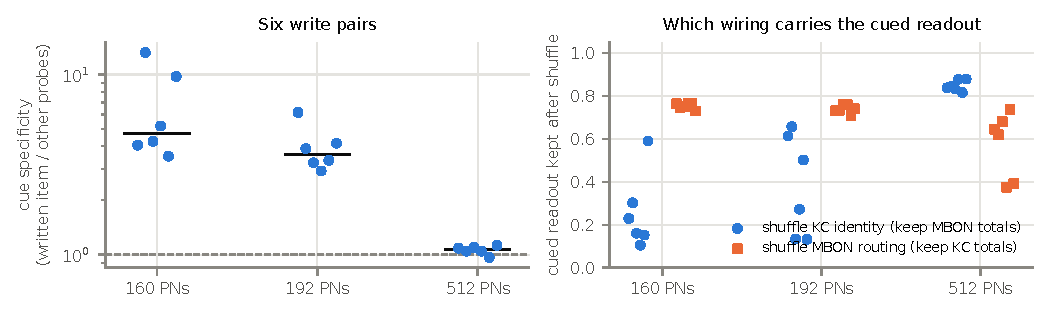
\includegraphics[width=0.95\textwidth]{figures/fig4_addressing.pdf}
\caption{Addressing on the MBON input current, six write pairs. Left: cue
specificity (bars: medians; dashed: no specificity). Right: fraction of the
cued readout magnitude kept after shuffling KC identity within each MBON
(circles) or MBON routing within each KC (squares); both shuffles preserve the
multiset of weight changes exactly.}
\label{fig:addr}\end{figure*}

\begin{table}[t]
\caption{Addressing on the MBON input current, six write pairs. Cue
specificity: $|I|$ for the written item over the mean of another item and a
neutral cue. Scrambles preserve the multiset of $\Delta w$ exactly.}
\label{tab:addr}\centering
\footnotesize\setlength{\tabcolsep}{3pt}
\begin{tabular}{@{}lccc@{}}\toprule
& $n_{PN}=160$ & 192 & 512\\\midrule
Cue specificity (median) & 4.7 & 3.6 & 1.06\\
KC-identity scramble, magnitude & 0.11--0.59 & 0.13--0.66 & 0.82--0.88\\
KC-identity scramble, cosine & 0.90--0.97 & 0.94--0.98 & 0.99--1.00\\
MBON-routing scramble, magnitude & 0.73--0.77 & 0.71--0.76 & 0.38--0.74\\
MBON-routing scramble, cosine & 0.72--0.75 & 0.72--0.75 & 0.44--0.74\\\bottomrule
\end{tabular}
\end{table}

\subsection{The cue needs only sparseness; the output identity needs the real wiring}
Replacing the PN$\rightarrow$KC wiring by degree-preserving or uniform random
wiring reproduced the KC sparseness, symbol overlap, cue specificity and
KC-identity dependence at every sparse operating point, with random or with
glomerulus-structured symbol codes. The real wiring did not increase cue
specificity: a pre-stated test (real above the null median in at least 75\% of
pairs in each of four glomerular-code settings) failed (4/8, 6/8, 6/8, 7/8
pairs), and with random symbol codes the real wiring's median cue specificity
over eight items (2.9) lay below that of all four nulls (3.0--6.6).

The identity of the output is a different matter (Table~\ref{tab:route},
Fig.~\ref{fig:route}). In the connectome, the MBON currents evoked by eight
different items have mean pairwise cosine 0.76, with 57--60\% of each item's
current in five MBONs. Randomising the KC$\rightarrow$MBON wiring raises the
cosine to 0.96--0.98 and spreads the current (top five MBONs: 27--29\%);
randomising the PN$\rightarrow$KC wiring raises it to 0.97--0.99. Cue
specificity is unchanged by either.

Controls that preserve structure locate what matters. Swapping whole KC output
profiles among KCs of the same annotated subtype \emph{and the same body side}
leaves distinctness intact (0.745--0.756 against 0.756--0.764), as does
permuting PN inputs among PNs of the same type and side (0.72--0.77). The same
swaps with the two sides mixed destroy it (0.90--0.95), and so does every
earlier control that mixed the sides. Neither individual KC wiring nor any
fine matching between a KC's inputs and outputs is required; body side and KC
subtype are. A static model that sums the connectome output profiles of each
item's written KCs, weighted by their activity, reproduces the simulated
distinctness (0.76 and 0.72 against 0.91--0.93 and 0.86--0.87 after
within-subtype swapping), so the network dynamics add little to this step.

What differs between items depends on the input code. The side-blind random
codes are balanced across the body midline to within a few percent
(standard deviation of the left share of PNs across 26 items: 0.03), but the
sparse KC threshold amplifies these small differences: the left share of the
KCs an item writes ranges from 0.04 to 0.95 (standard deviation 0.23--0.26),
and it predicts the left share of the MBON output ($r=0.96$). Items are then
stored largely in one of the two mushroom bodies. At dense input this
lateralisation disappears (0.43--0.56). Real odours activate homologous
glomeruli on both sides, so we repeated the analysis with bilaterally
symmetric glomerular codes (all PNs of a set of PN types). Lateralisation then
nearly vanishes (standard deviation 0.06--0.08), distinctness is reduced but
remains clearly above the nulls (0.88 against 0.96--0.99 for either
randomisation), and it now depends on KC subtype rather than on side:
swapping output profiles within subtype with sides mixed keeps it (0.90), while
keeping sides and mixing subtypes removes it (0.95--0.97). Items differ in the
KC subtypes they recruit (share of the written activity across items:
$\alpha\beta$ $0.42\pm0.15$, $\gamma$-main $0.36$--$0.38\pm0.11$,
$\alpha'\beta'$-ap1 $0.10$--$0.12\pm0.07$--$0.11$), and each subtype projects
to its own lobe's MBONs. Subtypes that receive little olfactory input in the
fly, $\gamma$-dorsal and $\alpha\beta$-posterior, were almost never recruited
($<0.3\%$), a sanity check on the PN wiring.

With a single teacher, the dopaminergic gate carries no item identity: across
items the per-MBON gate vectors were identical (cosine 1.000), clamping every
item's gate to the across-item mean left distinctness unchanged (0.756,
0.764), and replacing the gate by $+1$ on every gated MBON, which removes the
hand-set valence signs, changed it by at most 0.02.

The subtype-to-MBON map (Fig.~\ref{fig:map}) is block-structured and follows
the lobe organisation: $\alpha\beta$ KCs supply MBON14 and neighbouring
$\alpha$-lobe MBONs, $\alpha\beta$-posterior KCs supply MBON19,
$\alpha'\beta'$ subtypes supply MBON10/13/15/16/17/28, $\gamma$-main KCs supply
MBON01/05/21 and $\gamma$-dorsal KCs MBON27 (connectome annotation names).
Under bilateral codes, an item's KC-subtype mixture alone, combined with the
mean output profile of each subtype, explains 66\% of the item-to-item
variation of the output ($R^2=0.66$, 26 items).

\begin{figure*}[t]\centering
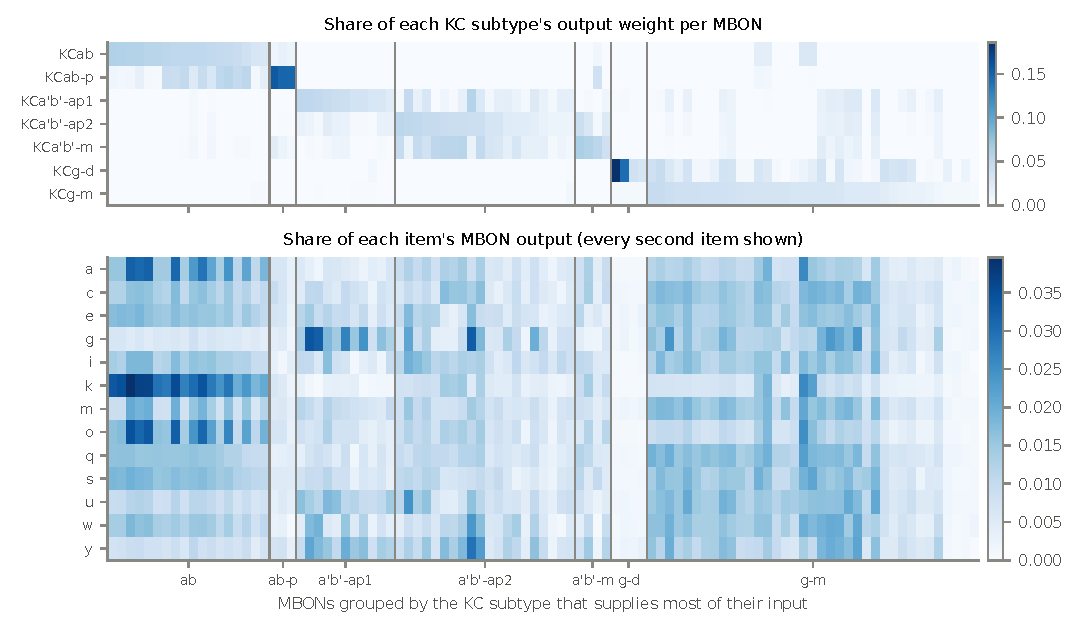
\includegraphics[width=0.95\textwidth]{figures/fig7_output_map.pdf}
\caption{Output map at 192 PNs with bilateral glomerular codes. Top: share of
each KC subtype's total output weight going to each MBON; MBONs are grouped by
the subtype that supplies most of their KC input. Bottom: share of each item's
output (activity-weighted sum of its written KCs' output profiles) per MBON,
for every second of 26 items.}
\label{fig:map}\end{figure*}

\subsection{When teachers differ, the teacher chooses the compartment}
Real memories are taught by different dopaminergic neurons. We wrote six items
with four teachers: all PAM, all PPL, and two halves of the PAM types
(PAM01--07, PAM08--15). The teachers produced different gates (cosine between
the two PAM halves 0.19; between PAM and PPL $-0.10$), and the same item written
by different teachers produced nearly unrelated outputs (cosine 0.085 between
the PAM halves, $-0.06$ between PAM and PPL). Across the 24 item--teacher
combinations, the teacher explained 87\% of the variance of the normalised
output, the item 5\%, and their interaction 7\%; within a teacher, items
remained as distinct as before (0.89--0.91). The dopaminergic system therefore
decides \emph{where} a memory is stored, and the KC layer decides what is
stored there and which cue retrieves it. The sign of the change is not a
result: in this model PAM writes potentiate and PPL writes depress (100\% of
changed synapses in each case) because of the hand-set valence signs, whereas
in the fly coincident KC and dopaminergic activity depresses KC$\rightarrow$MBON
synapses \cite{hige2015}. Re-running the location results with every DAN
depressing its compartment gave the same values (cue specificity 4.71, 3.59
and 1.07; item distinctness 0.885; teacher share 87\%). For single-teacher
norms and cosines this is largely guaranteed by symmetry, so the check mainly
shows that network feedback does not depend on the sign.

\subsection{Interference between memories is additive and set by KC overlap}
Writing a second item $Y$ after $X$ changed the cued readout of $X$ by exactly
the amount that $Y$'s write alone produces when read by cue $X$ (median
0.29 predicted and measured with the same teacher, 0.55 against 0.55 with
different teachers, 1.57 against 1.57 at dense input). Interference is linear
superposition in the weights, and its size follows the overlap between the KCs
$Y$ writes and those cue $X$ activates: 0.10--0.13 at sparse input against
0.86--0.90 at dense input, where $Y$'s contamination exceeds $X$'s own trace
1.6- to 2.9-fold. With the same teacher, the contamination lies along $X$'s own
output direction (cosine 0.999); with different teachers it adds a new
direction (0.88 sparse, 0.58 dense), because cue $X$ reads $Y$'s changes in
other compartments through shared KCs. Separate compartments thus do not
prevent interference; sparse KC codes do.

\begin{figure*}[t]\centering
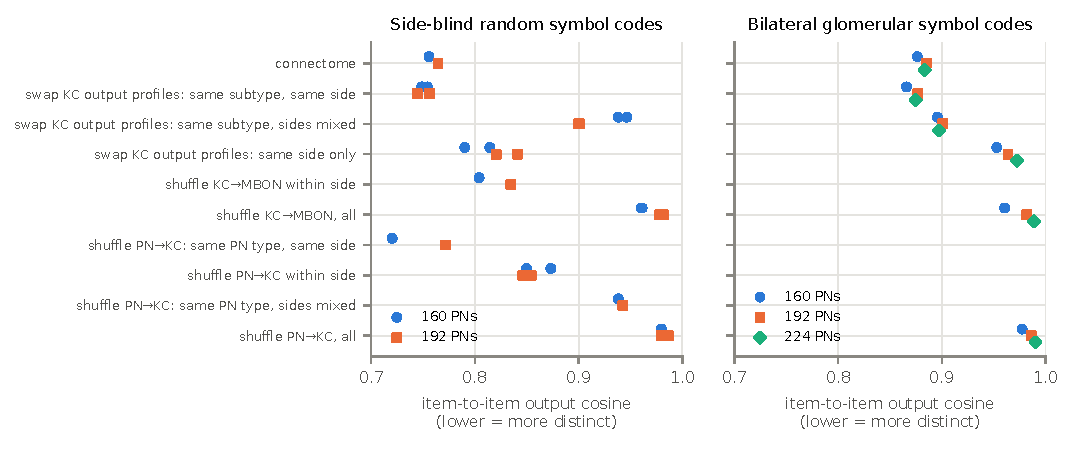
\includegraphics[width=0.95\textwidth]{figures/fig5_routing.pdf}
\caption{Item distinctness of the MBON output (mean pairwise cosine between
the input currents evoked by eight items; lower = more distinct) in the
connectome and under wiring nulls, for side-blind random symbol codes (left)
and bilaterally symmetric glomerular codes (right). One point per null draw.}
\label{fig:route}\end{figure*}

\begin{table}[t]
\caption{Item distinctness of the MBON output under rewiring, side-blind
random codes (8 items). Mean pairwise cosine between items' MBON currents;
ranges over null draws.}
\label{tab:route}\centering
\footnotesize\setlength{\tabcolsep}{3pt}
\begin{tabular}{@{}lcc@{}}\toprule
Wiring & $n_{PN}=160$ & 192\\\midrule
Connectome & 0.756 & 0.764\\
Swap profiles, same subtype and side & 0.749--0.754 & 0.745--0.756\\
Swap profiles, same side only & 0.79--0.81 & 0.82--0.84\\
Swap profiles, same subtype, sides mixed & 0.94--0.95 & 0.90\\
KC$\rightarrow$MBON shuffle within side & 0.80 & 0.83\\
KC$\rightarrow$MBON shuffle within class, sides mixed & 0.94 & 0.90--0.91\\
KC$\rightarrow$MBON shuffle, all & 0.96 & 0.98\\
PN$\rightarrow$KC shuffle, same PN type and side & 0.72 & 0.77\\
PN$\rightarrow$KC shuffle within side & 0.85--0.87 & 0.85\\
PN$\rightarrow$KC shuffle, same PN type, sides mixed & 0.94 & 0.94\\
PN$\rightarrow$KC shuffle, all, degree-preserving & 0.98 & 0.98--0.99\\
Dense input (512 PNs): connectome / shuffle & \multicolumn{2}{c}{0.91 / 0.95--0.96}\\\bottomrule
\end{tabular}
\end{table}

\subsection{Downstream neurons see the memory only through MBON spikes}
\label{sec:gating}
In the sparse regime the cued MBON response is mostly subthreshold (about one
MBON spike per probe), and central targets showed no change at the numerical
floor. Across 128 cells (four operating points, four levels of an added MBON
depolarising bias, four pairs, two probes), the central response differed from
the no-write response in all 31 cells in which the write changed the MBON spike
count and in all 4 in which it moved a spike without changing the count, and
in none of the 93 cells with identical MBON rasters (maximum change
$2.3\times10^{-7}$). Raising MBON excitability did not open this gate
reliably, because which threshold crossing flips is discrete. The memory is
therefore transmitted as a small number of added, removed or shifted MBON
spikes, which explains the step-like readout curves (Fig.~\ref{fig:gate}).

\begin{figure}[t]\centering
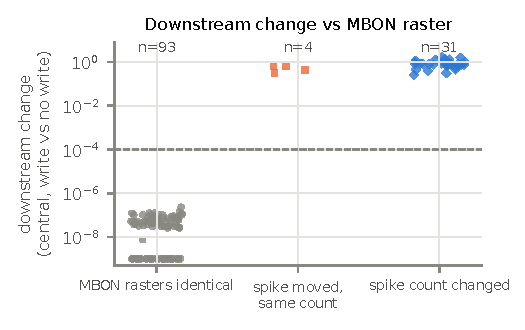
\includegraphics[width=\columnwidth]{figures/fig6_spike_gating.pdf}
\caption{Downstream (central) response change caused by the write, grouped by
whether the write changed the MBON spike raster (128 cells). Dashed: 1e-4.
Exact zeros are drawn at 1e-9.}
\label{fig:gate}\end{figure}

% =====================================================================
\section{Corrections to earlier analyses of this model}
\label{sec:corrections}
\begin{itemize}
\item \emph{Wrong-synapse writes.} Before a simulator fix on 2026-09-17, the
masked weight matrix was uploaded with unsorted column indices and re-sorted in
place by the first GPU matrix product, after the plasticity module had cached
its edge positions. In that state 61{,}164 of 61{,}210 cached positions point
to a different presynaptic cell (11{,}130 to non-KCs), and writing back the
unchanged weights alone alters the MBON input rows by 63\% (L2). The capacity
comparison of the earlier draft (frozen 1.17 against plastic 1.16) and the
earlier retention curves predate the fix. Re-run after the fix, the frozen
value reproduces (1.162--1.186 over three seeds) but plasticity
\emph{lowers} activity-based recall (1.126--1.131; paired differences $-0.034$
to $-0.056$), and the synaptic state carries history beyond the input window
(lags 4--12: 0.11--0.16) that activity does not (0.004--0.028).
\item \emph{Input echo.} The capacity task injected the previous three symbols
together with the current one; its lag-1 to lag-3 accuracies measure the input
window, not network memory.
\item \emph{Predictions true by construction.} The reported invariance of the
no-write response geometry to plasticity dose and delay holds because the
no-write branch performs no write and the network is silent during the delay.
The reported rescaling without rotation of the write state across gaps holds
because the gap applies a scalar decay.
\item \emph{An intermediate claim of this study, withdrawn.} An earlier version
of this analysis concluded that output identity required fine,
individual-level matching between each KC's inputs and outputs. That followed
from controls that all mixed the two hemispheres; side-preserving controls
(Table~\ref{tab:route}) show that body side and KC subtype suffice.
\item \emph{Dense operating point.} All earlier experiments used 512 of 675
PNs per symbol, where the KC code is dense; the reported probe-fixed direction
of the write effect and the near-collinearity of probe responses follow from
all probes activating nearly the same KCs.
\end{itemize}

% =====================================================================
\section{Discussion}
In this model, a mushroom-body memory has three addresses. The KC layer supplies
the retrieval key: when input is sparse, only a cue that re-activates the
written KCs retrieves the change, and random PN$\rightarrow$KC wiring suffices
for this, as expected from random-expansion accounts
\cite{caron2013,litwinkumar2017}. The output identity, in contrast, requires the
real wiring, but only its coarse organisation: which hemisphere, and which KC
subtype, a KC belongs to on both its input and its output side. Within a
subtype and a side, KCs are interchangeable, consistent with random
glomerulus-to-KC convergence \cite{caron2013}. An item's output is the sum of
the output profiles of the KCs it recruits, and items differ at the output to
the extent that they recruit different mixtures of mushroom bodies and of KC
subtypes, which the lobe-specific KC$\rightarrow$MBON organisation
\cite{aso2014a,li2020} maps onto different MBONs. How strongly they do so
depends on the input: side-blind codes produce strongly lateralised storage,
which is unlikely for real odours; bilaterally symmetric codes produce weaker,
subtype-based distinctness. Both addresses depend on an operating point with a
sparse KC code \cite{honegger2011,lin2014}; at dense input the MB collapses to
a set of per-MBON scalars and loses both. A third address is supplied by the
dopaminergic system: which DANs teach decides which compartments store the
memory, and when teachers differ this dominates the output (87\% of its
variance). The resulting division of labour is: the DAN chooses the
compartment, the KC subtype mixture and body side shape the output within the
compartments the DAN allows, and the identity of the written KCs is the key
that retrieves it.

Two properties are set by modelling choices rather than by the wiring. Memory
lifetime is exactly the prescribed synaptic decay, and the network contributes
no maintenance because it is silent between events; claims about forgetting or
consolidation require intrinsic activity, feedback plasticity or
DAN$\rightarrow$MBON dynamics that this model lacks \cite{eschbach2020}. And the
readout's all-or-none character follows from integrate-and-fire transmission:
downstream neurons see the memory only when it changes an MBON spike.

\paragraph*{Limitations}
One connectome and one reconstruction; leaky integrate-and-fire neurons with
hand-set gain, tonic drive and zero noise; a hand-set plasticity rule and
valence signs; symbol codes that are not odour responses; operating points
chosen by us; write pairs and items within one connectome as the only
replication; input current as a linear proxy that ignores spiking; the sparse
regime's memory is largely subthreshold at the MBON; symbol codes are either
side-blind or built from whole PN types, and neither is an odour response;
teachers are artificial pulses on whole DAN groups; the default sign of
plasticity (PAM potentiates, PPL depresses) is a model assumption opposite to
the fly's DAN-induced depression; location results were unchanged under a
depression-only rule, but the sign of stored changes is not interpretable. None of the results is a claim about memory in the
fly.

% =====================================================================
\section*{Data and code}
All scripts (\texttt{m1\_core.py} for the snapshot interface and one script
per experiment), their JSON outputs and a result register that maps each number
above to its output file are available at
\url{https://github.com/LxCenady/Fly-Is-All-You-Need}.

\begin{thebibliography}{99}
\bibitem{hige2015} T. Hige, Y. Aso, M. N. Modi, G. M. Rubin, and G. C. Turner,
``Heterosynaptic plasticity underlies aversive olfactory learning in
\textit{Drosophila},'' \textit{Neuron}, vol.~88, pp.~985--998, 2015.
\bibitem{aso2014a} Y. Aso \textit{et al.}, ``The neuronal architecture of the
mushroom body provides a logic for associative learning,'' \textit{eLife},
vol.~3, e04577, 2014.
\bibitem{modi2020} M. N. Modi, Y. Shuai, and G. C. Turner, ``The
\textit{Drosophila} mushroom body: from architecture to algorithm in a
learning circuit,'' \textit{Annu. Rev. Neurosci.}, vol.~43, pp.~465--484, 2020.
\bibitem{honegger2011} K. S. Honegger, R. A. A. Campbell, and G. C. Turner,
``Cellular-resolution population imaging reveals robust sparse coding in the
\textit{Drosophila} mushroom body,'' \textit{J. Neurosci.}, vol.~31,
pp.~11772--11785, 2011.
\bibitem{lin2014} A. C. Lin, A. M. Bygrave, A. de Calignon, T. Lee, and G.
Miesenb\"ock, ``Sparse, decorrelated odor coding in the mushroom body enhances
learned odor discrimination,'' \textit{Nat. Neurosci.}, vol.~17,
pp.~559--568, 2014.
\bibitem{caron2013} S. J. C. Caron, V. Ruta, L. F. Abbott, and R. Axel,
``Random convergence of olfactory inputs in the \textit{Drosophila} mushroom
body,'' \textit{Nature}, vol.~497, pp.~113--117, 2013.
\bibitem{takemura2017} S.-y. Takemura \textit{et al.}, ``A connectome of a
learning and memory center in the adult \textit{Drosophila} brain,''
\textit{eLife}, vol.~6, e26975, 2017.
\bibitem{li2020} F. Li \textit{et al.}, ``The connectome of the adult
\textit{Drosophila} mushroom body provides insights into function,''
\textit{eLife}, vol.~9, e62576, 2020.
\bibitem{litwinkumar2017} A. Litwin-Kumar, K. D. Harris, R. Axel, H.
Sompolinsky, and L. F. Abbott, ``Optimal degrees of synaptic connectivity,''
\textit{Neuron}, vol.~93, pp.~1153--1164, 2017.
\bibitem{shiu2024} P. K. Shiu \textit{et al.}, ``A \textit{Drosophila}
computational brain model reveals sensorimotor processing,'' \textit{Nature},
vol.~634, pp.~210--219, 2024.
\bibitem{lappalainen2024} J. K. Lappalainen \textit{et al.},
``Connectome-constrained networks predict neural activity across the fly visual
system,'' \textit{Nature}, 2024.
\bibitem{eschbach2020} C. Eschbach \textit{et al.}, ``Recurrent architecture
for adaptive regulation of learning in the insect brain,'' \textit{Nat.
Neurosci.}, vol.~23, pp.~544--555, 2020.
\bibitem{olddraft} Earlier draft of this study (2026-09-20), superseded;
see the correction register PAPER\_OVERTURN\_20260928.md.
\end{thebibliography}
\end{document}
